\section{TJ-Monopix1}
    %%%%%%%%%%%%%%%%%%%%%%%%%%%%%%%%%%%%%%%%
    %%  Slide 1: <READOUT>  %%
    %%%%%%%%%%%%%%%%%%%%%%%%%%%%%%%%%%%%%%%%
    \begin{frame}[noframenumbering]
        \frametitle{Front end electronics}
            \begin{columns}
                \column{0.7\textwidth}  
                Pitch$\sim$\SI{50}{\um} $\rightarrow$ \textbf{pixel area economy} and dimension of components are extremely relevant. \\\smallskip
                %MAPS usage allowed by miniaturization of components, i.e. TJ-Monopix1 is 180{nm} CMOS process.\\
                \column{0.4\textwidth}  
                    \begin{figure}[h!]
                        \vspace*{-0.9cm}\hspace*{-0.9cm}
                        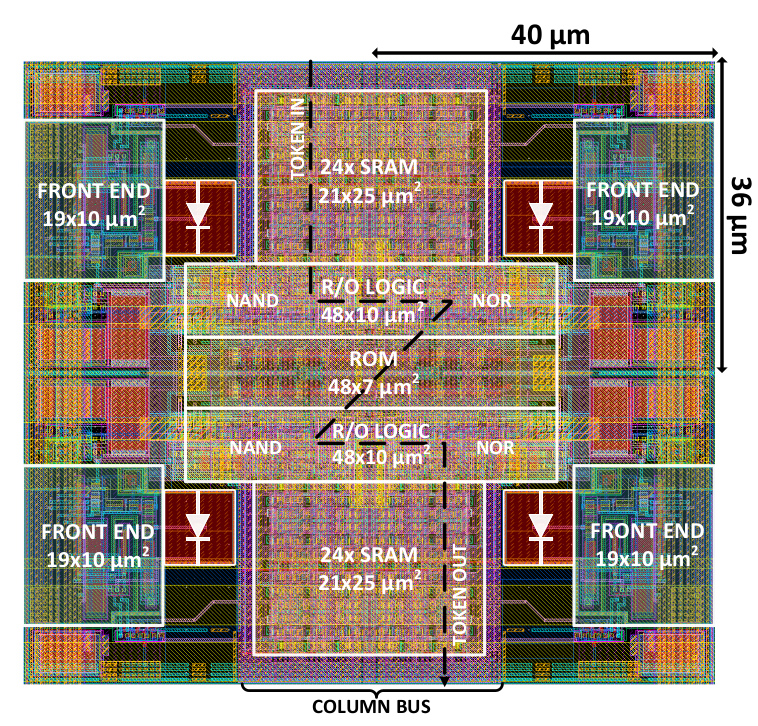
\includegraphics[width=1.06\linewidth]{figures/Monopix1/Monopix1_2x2pixelsgroup.png}
                    \end{figure}
            \end{columns}

            \begin{columns}
                \column{0.45\textwidth} 
                    The pixel area include the:
                    \begin{itemize}
                        \item Analog front end
                        \item Digital readout 
                    \end{itemize} 
                \column{0.55\textwidth} 
                    \vspace*{-0.15cm}%\hspace*{+0.15}
                    \begin{beamercolorbox}[rounded=true, center]{palette light primary}
                        \setlength{\tabcolsep}{0.5em} % for the horizontal padding
                        {\renewcommand{\arraystretch}{1.2}% for the vertical padding
                        \begin{tabular}{l|l}
                            \circled{Analog} & Digital\\
                            \hline
                            Triggered & \circled{Triggerless}\\
                            \hline
                            Buffer & \circled{No buffer} \\
                            \hline
                            Rolling shutter & \circled{Sparsified}\\
                        \end{tabular}
                        }
                    \end{beamercolorbox}
            \end{columns}
    \end{frame} 



    %%%%%%%%%%%%%%%%%%%%%%%%%%%%%%%%%%%%%%%%
    %%  Slide 1: <TJ-Monopix1>  %%
    %%%%%%%%%%%%%%%%%%%%%%%%%%%%%%%%%%%%%%%%
    \begin{frame}
        \frametitle{TowerJazz Monopix1}
        \begin{itemize}
            \item Designed by ATLAS collaboration
            \item Produced by TowerJazz, an electronic foundry located in Israel
            \item Small electrode design: \SI{2}{\um} with C=\SI{3}{fF}
            \item The sensor implements a process modification in the epi-layer that allows the creation of a planar junction (ALICE)
            \item The Front End has 4 flavors, all ALPIDE-like (ALPIDE chip design by ALICE and used in the ITS2)
        \end{itemize}
        \begin{columns}
            \column{0.5\textwidth}  
                \begin{table}
                    \begin{tabular}{| c |c |}
                    \hline
                    Resistivity & $>$\SI{1}{k\ohm cm}\\
                    Matrix size &  1$\times$2\si{cm\squared}\\
                    Pixel size & 36 $\times$ 40 \si{\um\squared}\\
                    Max depletion & \SI{25}{\um}\\
                    Time resolution & \SI{25}{ns} \\
                    %Power cons. & $\sim$ 120 \si{mW/cm\squared}\\    
                    \hline
                    \end{tabular}
                \end{table}
            \column{0.5\textwidth} 
                \hspace*{-0.4cm}\includegraphics[width=1.1\linewidth]{figures/Monopix1/Monopix1_section_scheme_ngap.png}\\
        \end{columns}
    \end{frame} 


    %%%%%%%%%%%%%%%%%%%%%%%%%%%%%%%%%%%%%%%%
    %%  Slide 1: <TJ-Monopix1>  %%
    %%%%%%%%%%%%%%%%%%%%%%%%%%%%%%%%%%%%%%%%
    \begin{frame}
        \frametitle{TJ-Monopix1 analog output}
        \begin{columns}
            \column{0.5\textwidth}
            ToT = \textbf{Time Over Threshold}\\
            \bigskip
            \hspace*{-0.5cm} 
                \includegraphics[width=1.25\linewidth]{figures/Monopix1/tot_example.pdf}
            \column{0.5\textwidth}  
                \begin{itemize}
                    \item The reset circuit of the amplifier made with a \textbf{PMOS}, guaranties the discharge of the preamplifier with constant slope
                    \item The ToT grows linearly with the pulse amplitude
                    \item Before readout ToT is stored in RAM as a 6-bits variable $\rightarrow$ then the ToT can vary in range 0-\SI{1.6}{\us}
                \end{itemize}
        \end{columns}
    \end{frame} 



 







